\appendix
\clearpage
\addappheadtotoc
\appendixpage
\chapter{Detalles Técnicos}
A veces, después de la investigación realizada a través de años de nuestro trabajo académico, contamos con mucho material que complementan nuestro artículo académico. Este material podría distraer o ser inapropiado en el cuerpo del manuscrito. 

\begin{center}
\begin{table}[!ht]
\centering
\caption{Datos de ...}

\begin{tabular}{ !{\vrule width 1pt}c!{\vrule width 1pt}c!{\vrule width 1pt}}
\noalign{\hrule height 1pt}
\cellcolor[gray]{0.9} \textbf{Año} &
\cellcolor[gray]{0.9} \textbf{Porcentaje}
\\ \noalign{\hrule height 1pt}
2000 & $0.29\%$
\\ \hline
2001 & $0.45\%$
\\ \hline
2002 & $0.68 \%$
\\ \hline
2003 & $1.01 \%$
\\ \hline
2004 & $1.47 \%$
\\ \hline
2005 & $5.48 \%$
\\ \noalign{\hrule height 1pt}
\end{tabular}
%\label{table:moneda}
\end{table}
\end{center}


\section{Correlación} 
\begin{figure}[!h]
	\centering
\caption{\label{fig:correlacion}Correlación de las Variables}
	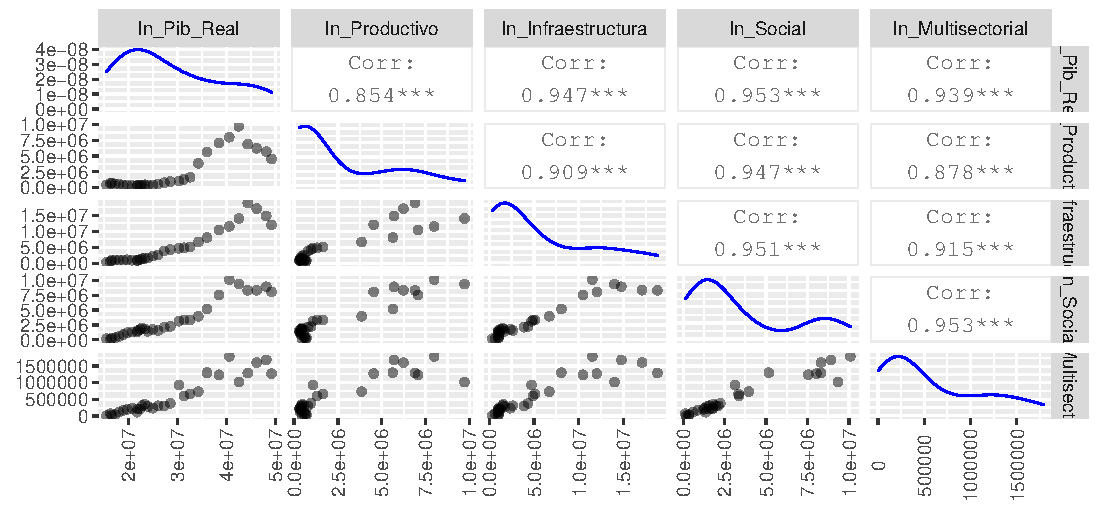
\includegraphics[scale=0.7]{Imagenes/correlacion1.pdf}	
\end{figure}

\chapter{Pruebas de Robustez}
En general, un apéndice es apropiado para materiales que son relativamente breves y que se presentan fácilmente en formato impreso. Algunos ejemplos de material adecuado para un apéndice son:

\begin{table}[!hbt]
\centering
\caption{ Como Realizar un Cuadro }
\begin{tabular}{|c|l|r|r|}
\hline N& Item& Precio& Cantidad\\
\hline \rowcolor{red}[0.9\tabcolsep]
\rule{0pt}{2.9ex}\noindent 1& A& 35& 140\\
\hline \rowcolor[gray]{0.7}[0.91\tabcolsep]
\rule{0pt}{2.7ex}\noindent 2& B& 55& 55\\
\hline \rowcolor{green}[0.91\tabcolsep]
\rule{0pt}{2.7ex}\noindent 3& C & 75& 75\\
\hline \multicolumn{3}{|r|}{Total}&
\cellcolor{blue} 270\\
\hline
\end{tabular}
\end{table}

\centering
\tcbox[left=0pt,right=0pt,top=0.5ex,bottom=0pt,boxsep=0pt,
toptitle=0.5ex,bottomtitle=0.5ex,title=Muestra de Tabla]{

\begin{tabular}[t]{rl}
Numero 1 & 100 \\
Numero 2 & 100 \\
Numero 3 & 150 \\
Sum & 350
\end{tabular}}